\documentclass[11pt,a4paper]{article}
\usepackage[utf8]{inputenc}
\usepackage[french]{babel}
\usepackage[T1]{fontenc}
\usepackage{mathtools}
\usepackage{tikz}
\usepackage{amsmath, amssymb, amsthm}            
\usepackage{amstext, amsfonts, a4}
\usepackage{hyperref}
\usepackage[ruled,vlined, french, onelanguage]{algorithm2e}
\usepackage[left=2cm,right=2cm,top=2cm,bottom=2cm]{geometry}
\usepackage{multicol}
\usepackage{xcolor}

\usepackage{lscape}


\def\ccB{\mathscr{B}}
\newcommand\numberthis{\addtocounter{equation}{1}\tag{\theequation}}


\begin{document}
\section{Introduction}
Dans ce document on s'intéresse à la discrétisation du Laplacien pour un problème type Laplace
\begin{equation}
-\Delta\,u = F \label{eq:laplace}
\end{equation}
sur des maillages simples.

\section{Second ordre en 1D}
\begin{figure}[h]
\centering
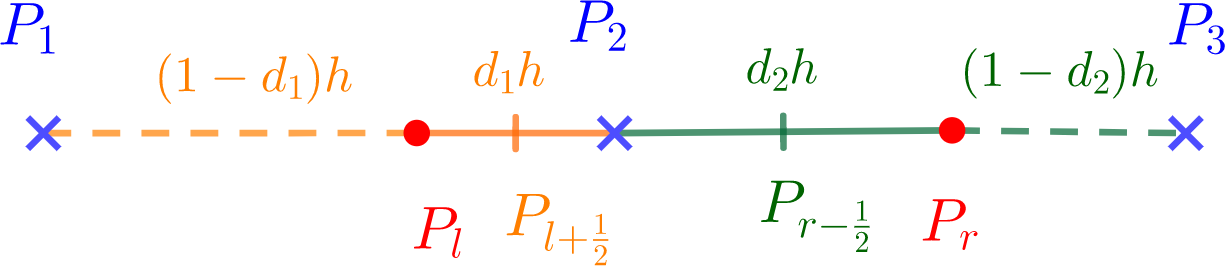
\includegraphics[width=0.7\textwidth]{secondOrdre1D.png}
\caption{Illustration : 1D}
\end{figure}

En une dimension, le problème de Laplace $\eqref{eq:laplace}$ est discrétisé sous la forme 
\begin{equation}
-\frac{u_{i-1} - 2\,u_i + u_{i+1}}{h^2} = f_i
\end{equation}
Sur une grille cartésienne quelconque où tous les points sont à une distance $h$ de leurs voisins directs et sous des conditions aux limites périodiques, résoudre $\eqref{eq:laplace}$ revient à résoudre le système linéaire suivant
\begin{equation}
\left[\begin{matrix}
a & b & &b \\
b & \ddots & \ddots &\\
& \ddots & \ddots & b\\
b& & b & a
\end{matrix}\right]\,U = F
\end{equation}
avec $a:= -2b$ et $b:=-\frac{1}{h^2}$.\\

Dans l'exemple illustré \textbf{Figure 1} le système est encore plus simplifié si l'on considère uniquement les points $P_1, P_2$ et $P_3$ comme étant des points de grille :
\begin{equation}
\left[\begin{matrix}
a & b & b\\
b & a & b\\
b & b & a
\end{matrix}\right]\,\left(\begin{array}{c}
u_1\\
u_2\\
u_3
\end{array}\right) = \left(\begin{array}{c}
f_1\\
f_2\\
f_3
\end{array}\right)
\end{equation}

Maintenant imaginons que nous voulions rajouter des points supplémentaires sur ce maillage, pour pouvoir, par exemple, imposer des conditions aux limites supplémentaires plus tard.\\

\noindent On introduit ainsi les points $P_r$ et $P_l$ :
\begin{itemize}
\item $P_l$ étant à une distance de $(1-d_1)h$ de $P_1$ et à une distance de $d_1h$ de $P_2$.
\item $P_r$ étant à une distance de $(1-d_2)h$ de $P_2$ et à une distance de $d_2h$ de $P_3$.
\end{itemize}

\subsection{$P_l$}

Dans un premier temps, analysons la discrétisation du Laplacien en 1D sur un maillage non régulier :
\begin{align*}
\Delta\,u &= \partial_x^2\,u = \partial_x (\partial_x u)
\end{align*}
Étudions dans un premier temps les développement de Taylor autour de $P_l$
\begin{align*}
u \left(P_1\right) &= u \left(P_l-\left(1-d_1\right)h\right) = u \left(P_l\right) - \left(1-d_1\right)h\,u'\left(P_l\right) + \frac{\left(1-d_1\right)^2h^2}{2}\,u''(P_l) + O\left(\left(1-d_1\right)^3h^3\right)\\
u (P_2) &= u \left(P_l+d_1h\right) = u \left(P_l\right) + d_1h\,u'\left(P_l\right) + \frac{d_1^2h^2}{2}\,u''\left(P_l\right) + O\left(d_1^3h^3\right)\\
\end{align*}

On peut remarquer que 
\begin{equation}
d_1u \left(P_1\right) - d_1u\left(P_l\right) - (1-d_1)u\left(P_l\right) + \left(1-d_1\right) u (P_2) = d_1(1-d_1)h\frac{h}{2}u''\left(P_l\right) + O(h^3)
\end{equation}
qui se réécrit comme
\begin{equation}
\lim_{h\to0}\frac{\frac{u(P_1)- u (P_l)}{(1-d_1)h} - \frac{u (P_l) - u (P_2)}{d_1h}}{\frac{h}{2}} = u''(P_l)
\end{equation}

\subsection{$P_r$}
De la même manière nous avons un développement de Taylor autour de $P_r$
\begin{align*}
u \left(P_3\right) &= u \left(P_r+\left(1-d_2\right)h\right) = u \left(P_r\right) + \left(1-d_2\right)h\,u'\left(P_r\right) + \frac{\left(1-d_2\right)^2h^2}{2}\,u''(P_r) + O\left(\left(1-d_2\right)^3h^3\right)\\
u (P_2) &= u \left(P_r-d_2h\right) = u \left(P_r\right) - d_2h\,u'\left(P_r\right) + \frac{d_2^2h^2}{2}\,u''\left(P_r\right) + O\left(d_2^3h^3\right)\\
\end{align*}
Qui conduit à
\begin{equation}
d_2u \left(P_2\right) - d_2u\left(P_2\right) - (1-d_2)u\left(P_r\right) + \left(1-d_2\right) u (P_3) = d_2(1-d_2)h\frac{h}{2}u''\left(P_r\right) + O(h^3)
\end{equation}
et qui se réécrit comme
\begin{equation}
\lim_{h\to0}\frac{\frac{u(P_2)- u (P_r)}{d_2h} - \frac{u (P_r) - u (P_3)}{(1-d_2)h}}{\frac{h}{2}} = u''(P_r)
\end{equation}
Nous avons donc deux nouvelles formules de discrétisation
\begin{align*}
&-\frac{2}{(1-d_1)h^2}\,u(P_1) + \frac{2}{h^2}\left( \frac{1}{1-d_1} + \frac{1}{d_1}\right)u(P_l) - \frac{2}{d_1h^2}\,u(P_2) = f_l\\
\Longleftrightarrow& \frac{2}{(1-d_1)}\,b\,u(P_1) -2b\left(\frac{1}{1-d_1} + \frac{1}{d_1}\right)u(P_l) + \frac{2}{d_1}b\,u(P_2) = f_l\\
\intertext{et}
&-\frac{2}{(1-d_2)h^2}\,u(P_3) + \frac{2}{h^2}\left( \frac{1}{1-d_2} + \frac{1}{d_2}\right)u(P_r) - \frac{2}{d_2h^2}\,u(P_2) = f_r\\
\Longleftrightarrow& \frac{2}{(1-d_2)}\,b\,u(P_3) -2b\left(\frac{1}{1-d_2} + \frac{1}{d_2}\right)u(P_r) + \frac{2}{d_2}b\,u(P_2) = f_r\\
\end{align*}

\subsection{$P_1$}
Vérifions maintenant que les coefficients calculés interviennent aussi dans la discrétisation du Laplacien au point $P_1$.\\
Nous avons un développement de Taylor autour de $P_1$
\begin{align*}
u (P_3) &= u \left(P_1-h\right) = u \left(P_1\right) - h\,u'\left(P_1\right) + \frac{h^2}{2}\,u''\left(P_1\right) + O\left(h^3\right)\\
u \left(P_l\right) &= u \left(P_1+(1-d_1)h\right) = u \left(P_1\right) + (1-d_1)h\,u'\left(P_1\right) + \frac{(1-d_1)^2h^2}{2}\,u''(P_1) + O\left((1-d_1)^3h^3\right)\\
\end{align*}
Qui conduit à
\begin{equation}
(1-d_1)u \left(P_3\right) - (1-d_1)u\left(P_1\right) - u\left(P_1\right) +  u (P_l) = (1-d_1)h\frac{(2-d_1)h}{2}u''\left(P_1\right) + O(h^3)
\end{equation}
et qui se réécrit comme
\begin{equation}
\lim_{h\to0}\frac{\frac{u(P_3)- u (P_1)}{h} - \frac{u (P_1) - u (P_l)}{(1-d_1)h}}{\frac{(2-d_1)h}{2}} = u''(P_1)
\end{equation}
La nouvelle formule de discrétisation en $P_1$ est donc
\begin{align*}
& \frac{2}{(2- d_1)h^2}u(P_3) - \frac{2}{h^2}\frac{1}{2-d_1}\left(1 - \frac{1}{1-d_1}\right)\,u(P_1) + \frac{2}{(2-d_1)(1-d_1)h^2}u(P_l) = f_1\\
& \Longleftrightarrow \frac{2}{2-d_1}b\,u(P_3) - 2b\frac{1}{2-d_1}\left(1- \frac{1}{1-d_1}\right)\,u(P_1) + \frac{2}{(2-d_1)(1-d_1)}b\,u(P_l) = f_1
\end{align*}

\subsection{$P_2$}
Vérifions maintenant que les coefficients calculés interviennent aussi dans la discrétisation du Laplacien au point $P_2$.\\
Nous avons un développement de Taylor autour de $P_2$
\begin{align*}
u (P_l) &= u \left(P_2-d_1h\right) = u \left(P_2\right) - d_1h\,u'\left(P_2\right) + \frac{d_1^2h^2}{2}\,u''\left(P_2\right) + O\left(d_1^3h^3\right)\\
u \left(P_r\right) &= u \left(P_2+d_2h\right) = u \left(P_2\right) + d_2h\,u'\left(P_2\right) + \frac{d_2^2h^2}{2}\,u''(P_2) + O\left(d_2^3h^3\right)\\
\end{align*}
Qui conduit à
\begin{equation}
d_2u \left(P_l\right) - d_2u\left(P_2\right) - d_1u\left(P_2\right) + d_1 u (P_r) = d_2d_1h\frac{(d_1+d_2)h}{2}u''\left(P_2\right) + O(h^3)
\end{equation}
et qui se réécrit comme
\begin{equation}
\lim_{h\to0}\frac{\frac{u(P_l)- u (P_2)}{d_1h} - \frac{u (P_2) - u (P_r)}{d_2h}}{\frac{(d_1+d_2)h}{2}} = u''(P_r)
\end{equation}
La nouvelle formule de discrétisation en $P_2$ est donc
\begin{align*}
& \frac{2}{(d_1 + d_2)d_1h^2}u(P_l) - \frac{2}{h^2}\frac{1}{d_1 + d_2}\left(\frac{1}{d_2} - \frac{1}{d_1}\right)\,u(P_2) + \frac{2}{(d_1 + d_2)d_2h^2}u(P_r) = f_2\\
& \Longleftrightarrow \frac{2}{(d_1+d_2)d_1}b\,u(P_l) - 2b\frac{1}{d_1 + d_2}\left(\frac{1}{d_2} - \frac{1}{d_1}\right)\,u(P_2) + \frac{2}{(d_1+d_2)d_2}b\,u(P_r) = f_2
\end{align*}

\subsection{$P_3$}
Vérifions maintenant que les coefficients calculés interviennent aussi dans la discrétisation du Laplacien au point $P_3$.\\
Nous avons un développement de Taylor autour de $P_3$
\begin{align*}
u (P_r) &= u \left(P_3-(1-d_2)h\right) = u \left(P_3\right) - (1-d_2)h\,u'\left(P_3\right) + \frac{(1-d_2)^2h^2}{2}\,u''\left(P_3\right) + O\left((1-d_2)^3h^3\right)\\
u \left(P_1\right) &= u \left(P_3+h\right) = u \left(P_3\right) + h\,u'\left(P_3\right) + \frac{h^2}{2}\,u''(P_3) + O\left(h^3\right)\\
\end{align*}
Qui conduit à
\begin{equation}
u \left(P_r\right) - u\left(P_3\right) - (1-d_2)u\left(P_1\right) +  (1-d_2)u (P_1) = (1-d_2)h\frac{(2-d_2)h}{2}u''\left(P_3\right) + O(h^3)
\end{equation}
et qui se réécrit comme
\begin{equation}
\lim_{h\to0}\frac{\frac{u(P_r)- u (P_3}{(1-d_2)h} - \frac{u (P_3) - u (P_1)}{h}}{\frac{(2-d_2)h}{2}} = u''(P_3)
\end{equation}
La nouvelle formule de discrétisation en $P_1$ est donc
\begin{align*}
& \frac{2}{(2- d_2)(1-d_2)h^2}u(P_r) - \frac{2}{h^2}\frac{1}{2-d_2}\left(\frac{1}{1-d_1} - 1\right)\,u(P_3) + \frac{2}{(2-d_2)h^2}u(P_1) = f_3\\
& \Longleftrightarrow \frac{2}{(2-d_2)(1-d_2)}b\,u(P_r) - 2b\frac{1}{2-d_2}\left(\frac{1}{1-d_2} - 1\right)\,u(P_3) + \frac{2}{(2-d_2)}b\,u(P_1) = f_3
\end{align*}

\subsection{Final}
\begin{figure}[h]
\centering
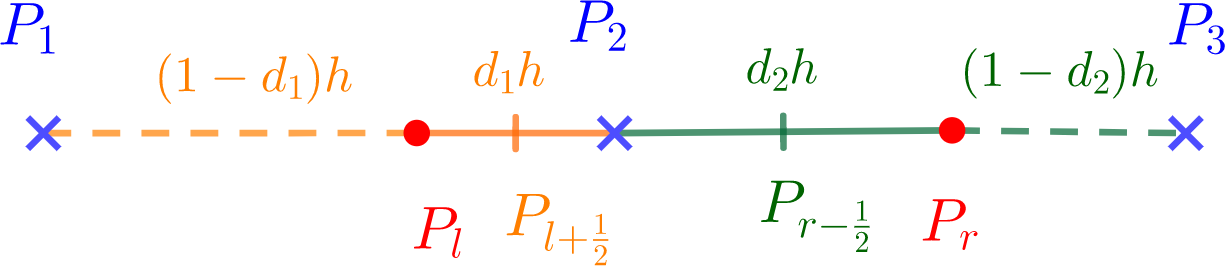
\includegraphics[width=0.4\textwidth]{secondOrdre1D.png}
\caption{Illustration : 1D}
\end{figure}
Maintenant nous avons donc 
\begin{align*}
\intertext{Pour $P_1$}
&2b\textcolor{red}{\frac{1}{2-d_1}}\,u(P_3) &-2b\textcolor{red}{\frac{1}{2-d_1}}\left(1- \textcolor{orange}{\frac{1}{1-d_1}}\right)\,u(P_1) &+2b \frac{1}{\textcolor{red}{(2-d_1)}\textcolor{orange}{(1-d_1)}}\,u(P_l) &= f_1\\
\intertext{Pour $P_2$}
&2b\frac{1}{\textcolor{pink}{(d_1+d_2)}\textcolor{green}{d_1}}\,u(P_l) &-2b\textcolor{pink}{\frac{1}{d_1 + d_2}}\left(\textcolor{cyan}{\frac{1}{d_2}} - \textcolor{green}{\frac{1}{d_1}}\right)\,u(P_2) &+2b \frac{1}{\textcolor{pink}{(d_1+d_2)}\textcolor{cyan}{d_2}}\,u(P_r) &= f_2
\intertext{Pour $P_3$}
&2b\frac{1}{\textcolor{brown}{(2-d_2)}\textcolor{purple}{(1-d_2)}}\,u(P_r) &- 2b\textcolor{brown}{\frac{1}{2-d_2}}\left(\textcolor{purple}{\frac{1}{1-d_2}} - 1\right)\,u(P_3) &+ 2b\textcolor{brown}{\frac{1}{(2-d_2)}}\,u(P_1) &= f_3
\intertext{Pour $P_l$}
&2b\textcolor{orange}{\frac{1}{1-d_1}}\,u(P_1) &-2b\left(\textcolor{orange}{\frac{1}{1-d_1}} - \textcolor{green}{\frac{1}{d_1}}\right)u(P_l) &+ 2b\textcolor{green}{\frac{1}{d_1}}\,u(P_2) &= f_l
\intertext{Pour $P_r$}
&2b\textcolor{purple}{\frac{1}{(1-d_2)}}\,u(P_3) &-2b\left(\textcolor{purple}{\frac{1}{1-d_2}} - \textcolor{cyan}{\frac{1}{d_2}}\right)u(P_r) &+ 2b\textcolor{cyan}{\frac{1}{d_2}}\,u(P_2) &= f_r
\end{align*}
\subsection{Formule générale}
\noindent Ainsi si on prend trois points alignés $a$, $b$ et $c$, séparés respectivement par des distances $d_{ab}$ et $d_{bc}$, alors la discrétisation 1D du Laplacien est
\begin{align*}
[\Delta]\,u (b) =\frac{\frac{u(a) - u(b)}{d_{ab}} - \frac{u(b) - u (c)}{d_{bc}}}{\frac{d_{ab}+d_{bc}}{2}}
\end{align*}
%\section{Second ordre en 2D}
%\begin{figure}[h]
%\centering
%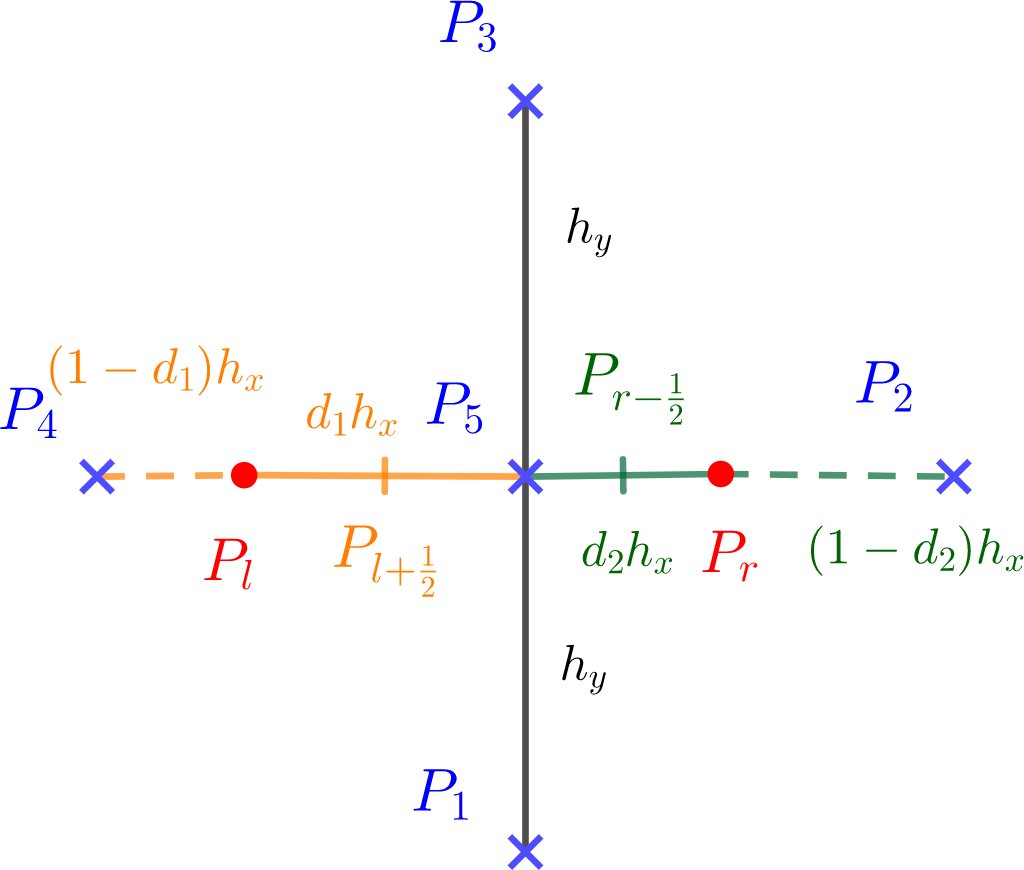
\includegraphics[width=0.4\textwidth]{secondOrdre2D.png}
%\caption{Illustration : 2D}
%\end{figure}


\end{document}